This section describes the various systematic uncertainties considered in the analysis, including uncertainties on both the jet and calorimeter clusters objects.
The uncertainties are broadly categorized into three classes: calibration, selection efficiency, and unfolding uncertainties. 
The calibration and selection efficiency uncertainties are studied for the jet and calorimeter clusters independently and then propagated through the full unfolding procedure, while the unfolding uncertainties are studied for the combined jet and calorimeter cluster response. 
This independent treatment is well-motivated given that the dominant uncertainty contributions arise from the hadronic response and noise threshold effects on the low-energy calorimeter clusters, which are less precisely constrained than the jet energy scale and resolution for jets with reconstructed $p_{T} > 21$ GeV.
All variations are evaluated both upward and downward, with the exception of the unfolding, pileup correction, and cluster resolution uncertainties, which are one-sided and not symmetrized. The overall uncertainty is dominated by the hadronic response and noise threshold variations.
The full set of systematic uncertainties with details on their evaluation in the analysis chain are listed in Table \ref{table:full_systematics}. 
Further details on the determination of each systematic uncertainty is given in the following sections. \newline
\begin{table}[ht]
\centering
\begin{tabular}{|c|c|c|c|}
\hline
Systematic Uncertainty & Type & Data/Sim Varied \\ \hline
JES Uncertainty & Calibration & Simulation \\ \hline
JER Uncertainty & Calibration & Simulation \\ \hline
Jet trigger efficiency & Selection efficiency & Data \\ \hline
Calorimeter tower calibration & Calibration & Data \\ \hline
Calorimeter tower resolution & Calibration & Simulation \\ \hline
Calorimeter hadronic response & Calibration & Data \\ \hline
Topocluster noise threshold & Selection efficiency & Data \& Sim \\ \hline
Pileup correction & Selection efficiency & Data \\ \hline
MBD vertex efficiency & Selection efficiency & Data \\ \hline
Prior reweighting & Unfolding & Simulation \\ \hline
Herwig response & Unfolding & Simulation \\ \hline
\end{tabular}
\caption{Full set of systematic uncertainties for underlying event measurement.}
\end{table}
\label{table:full_systematics}

\subsection{Jet Systematic Uncertainties}
The jet systematic uncertainties include the Jet Energy Scale (JES) uncertainty, the Jet Energy Resolution (JER) uncertainty and the jet trigger efficiency uncertainty.
The JES uncertainty is derived from the scale difference between data and MC in the in-situ photon-jet and multi-jet balance calibration studies~\cite{in_situ_note} and results in a $p_{T}$-independent 2.5\% uncertainty on the jet energy scale. 
The JER uncertainty is derived from the differences in JER results extracted from two different data-driven methods, the dijet balance method and the bisector method and results in a 1.8\% uncertainty on the jet energy resolution~\cite{ppg08AN}.
The jet trigger efficiency is derived by varying the fit parameters of the jet trigger efficiency fit function outlined in Section~\ref{sec:jet_trigger_eff} to find the 1$\sigma$ variations on the parameterized jet trigger efficiency. The jet trigger efficiency uncertainty is found to be negligible for the UE measurement with variations at the $<$ 1\% level.

\subsection{Calorimeter Cluster Systematic Uncertainties}

\subsubsection{Calorimeter cluster energy scale}
The absolute energy scale calibration uncertainties of the calorimeter towers for both the EMCal and HCals are determined from the uncertainties in the calorimeter calibration methodology \cite{ppg03AN,EMCal_calib_internal_note}.
A 0.5\% systematic uncertainty on the overall scale of the EMCal absolute energy calibration is applied to the EMCal towers included in the topoclusters. 
This uncertainty is based on the range in calibration values from toy MC studies of the mass and width of the $\pi^{0}$ and $\eta$ peaks ~\cite{jaeboem_emcal_calib}.
A 1\% systematic uncertainty on the overall scale of the OHCal absolute energy calibration is applied to OHCal towers included in the topoclusters. 
This uncertainty is based on the residual run dependence of the OHCal calibration in Run 2024~\cite{HCal_calib_internal_note}.
A 10\% systematic uncertainty on the overall scale of the IHCal absolute energy calibration is applied to the IHCal towers included in the topoclusters. This uncertainty is based on the residual Data/MC differences in the \detdeta extracted from the IHCal-only result~\cite{ppg03AN}.
An additional $\eta$ dependent scale uncertainty ranging from $-10\%$ to $10\%$ is applied to the OHCal towers included in the topoclusters. This uncertainty is based on residual position dependent Data/MC differences in the OHCal-only \detdeta~\cite{ppg03AN}.
The explicit values used for this uncertainty are extracted from the MC/Data ratio of the OHCal-only \detdeta measurement using Run 2024 Au+Au data and the \ampt simulation samples discussed in Section~\ref{sec:detdeta_mcsamples}.
The uncertainty values are determined as a function of OHCal $i\eta$ bin across the full detector acceptance and are shown in Figure~\ref{fig:ohcal_eta_dep_scale_uncertainty}.
\begin{figure}
    \centering
    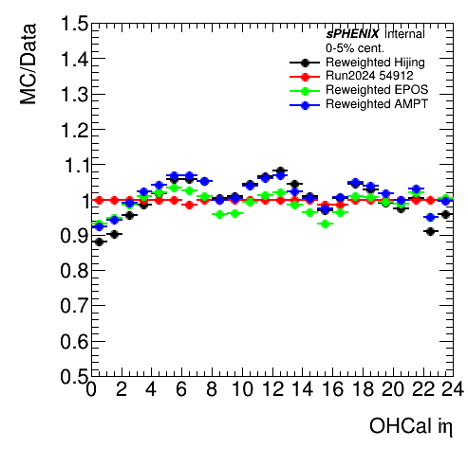
\includegraphics[width=0.7\linewidth]{ueinpp/Figures/systematics/eta_dependent_scale_uncertainty.png}
    \caption{Additional $\eta$ dependent scale uncertainty values as a function of OHCal $\eta$ tower index, $i\eta$, based on the Data/MC differences in the \detdeta extracted from the OHCal in \cite{ppg03AN}. Blue curve showing the MC/Data differences using \ampt is used for this scale uncertainty.}
    \label{fig:ohcal_eta_dep_scale_uncertainty}
\end{figure}
For all of these calorimeter tower calibration uncertainties, the overall scale of individual calorimeter towers included in the topoclusters is varied by the corresponding calibration uncertainty and this variation is then propagated through the unfolding procedure.
The overall effect of these calorimeter tower calibration uncertainties on the UE measurement is found to be at the 1\% level for all leading jet $p_T$ bins.

\subsubsection{Calorimeter hadronic response}
The uncertainty in the calorimeter hadronic energy scale is derived from Data/MC differences seen in the EMCal and HCal test beam paper~\cite{emcal_beamtest,emcal_hcal_beamtest}.
This uncertainty is the same as the hadronic response uncertainty applied to the \detdeta analysis~\cite{sphenix_detdeta} and outlined in more detail in Section~\ref{sec:detdeta_systematics} of this thesis.
The uncertainty is applied in the underlying event measurement by varying the overall scale of the topoclusters by 4.9\%, corresponding to the hadronic response uncertainty for energy in all three calorimeter layers, and this uncertainty is then propagated through the unfolding procedure.

\subsubsection{Calorimter cluster resolution}
The calorimeter cluster resolution uncertainty is constrained from the Data/MC differences seen in the EMCal clusters in toy MC studies of the mass and width of the $\pi^{0}$ and $\eta$ peaks~\cite{jaeboem_emcal_calib} at low energy ($E_{T} \sim 2-10$ GeV) and data-driven JER studies~\cite{ppg08AN} at high energy ($E_{T} > 15$ GeV).
Two different resolution variations are applied to the topoclusters used for the UE measurement: a variation on the position resolution of the topoclusters and a variation on the energy resolution of the topoclusters.

The position resolution of the topoclusters is varied by 0.005 radian. This uncertainty corresponds to the difference in position resolution factors between different toy MC models that were used to accurately fit both the mass and width of the $\pi^{0}$ and $\eta$ peaks in data and MC in the EMCal cluster calibration studies.
The variation in the position resolution of the topoclusters should have a negligible effect on the UE measurement as the UE measurement is summed over a large region of 2.2 units in $\eta$ and $2 \pi/ 3$ radians in $\phi$.
However, this variation is tested to check for any effects from flow of topoclusters in and out of the transverse region due to the position resolution of the topoclusters.
This uncertainty is applied by varying the position of the topoclusters in simulation by 0.005 radians and then propagating this uncertainty through the unfolding procedure.
The overall effect of this position resolution variation on the UE measurement is found to be negligible.

Two resolution studies are then used to constrain the calorimeter topocluster energy resolution uncertainty.
For both lower energy EMCal clusters and higher energy full calorimeter jets, the Data/MC differences in the resolution are found to be around 8-9\% with studies of the JER showing the majority of the Data/MC differences in resolution come from the EMCal contributions.
Therefore, the topocluster energy resolution differences between data and MC across the $E_{T}$ range in this analysis  are constrained by these two studies of the calorimeter resolution and an 8\% smearing on the topocluster energies is applied in simulation to find the cluster energy resolution systematic uncertainty on the UE measurement.
The total effect of this energy resolution variation on the on the UE measurement is also found to be at the $<$ 1\% level for all leading jet $p_T$ bins.

\subsubsection{Topocluster noise threshold}
The topocluster noise threshold are varied between the $2\sigma_{ped}$ and $4\sigma_{ped}$ clustering thresholds studied in the topocluster noise study in Section~\ref{sec:ueinpp_towerreco} to test the impact of the nominal noise threshold ($3\sigma_{ped}$) in the topocluster reconstruction on extracted calorimeter cluster total energy.
This variation is also sensitive to the reconstruction of low-energy particles by probing the extent to which real soft particles are included or excluded by the seeding requirements of the clustering procedure. 
In particular, varying the seeding requirements provides a test of the robustness of the truth-level results with respect to the reconstruction-level low-energy fiducial cut. 
By modifying the clustering thresholds, this study assesses the extent to which the final UE measurement depends on the inclusion or exclusion of soft particles near the fiducial boundary.
This uncertainty is applied by varying the topocluster noise threshold in both simulation and data and is propagated through the unfolding procedure with variations on both the measured histogram and the simulation response matrix.
The overall effect of this topocluster noise threshold variation on the UE measurement is found to be at the 3-4\% level when varying up and down to the $2\sigma_{ped}$ and $4\sigma_{ped}$ thresholds.

\subsubsection{Pileup correction}
The pileup correction is derived from the pileup correction study Section~\ref{sec:ueinpp_pileup} which shows the impact of pileup on the topocluster reconstruction and extracted calorimeter cluster total energy.
This pileup correction is applied to the reconstructed calorimeter cluster total energy to correct for the pileup effect and is propagated through the unfolding procedure as a variation on the data histogram.
To determine the impact of this pileup correction on the UE measurement, the pileup correction is toggled on and off.
The overall effect of the pileup correction on the UE measurement is found to be $< 3\%$ for all leading jet $p_T$ bins.

\subsubsection{MBD vertex efficiency}
To test the impact of using the simulation based MBD vertex efficiency applied in Section~\ref{sec:mbd_vertex_eff_app}, the MBD vertex efficiency differences in data and simulation are studied for a set of clean events, defined as events that pass the full suite of non collision background rejection cuts and have a leading jet with $\pT >$ 21 GeV and $\|\eta\| <$ 0.7.
Additionally, to limit any effects from the zvertex used in the jet reconstruction and any pileup effects, only 1.5mrad events where the zvertex width is narrower and pileup is low are used in this study.
Previous studies show that the zvertex effects on the average jet reconstruction transverse momentum as a function of zvertex position is negligible for events with zvertex within 60 cm of the nominal interaction point. 
However, large effects outside of this range are seen. 

The MBD vertex efficiency as a function of leading jet $\pT$ and transverse region $\Sigma E_{T}$ is shown in Figure~\ref{fig:mbd_vertex_efficiency_data_mc} for both data and simulation.
There is fairly good agreement between data and simulation in the MBD vertex efficiency with variations between 6-10\% across the leading jet $\pT$ and $<10\%$ across the transverse region $\Sigma E_{T}$ ranges studied.
The scale difference between data and simulation is taken as a systematic uncertainty on the simulation based MBD vertex efficiency. 
The overall effect of this MBD vertex efficiency systematic uncertainty on the UE measurement is found to be small $\sim 1\%$.
\begin{figure}
    \centering
    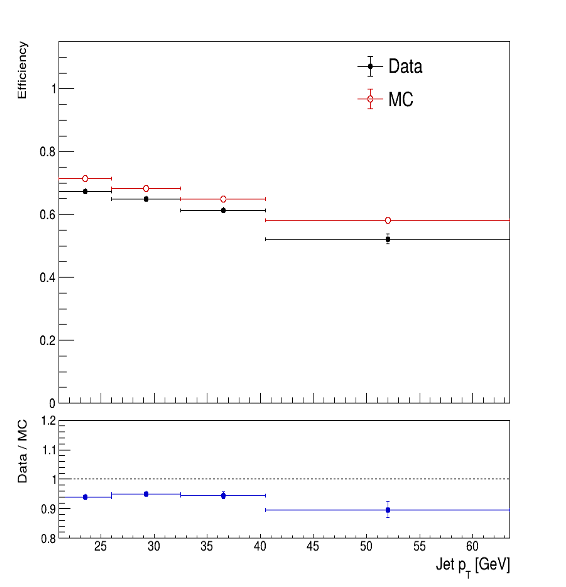
\includegraphics[width=0.48\linewidth]{ueinpp/Figures/mbd_vertex_efficiency/mbd_eff_mc_data_var_vs_jetpt.png}
    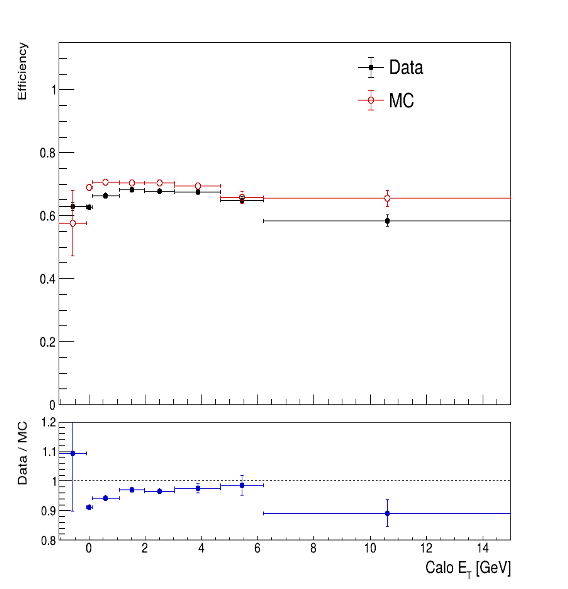
\includegraphics[width=0.48\linewidth]{ueinpp/Figures/mbd_vertex_efficiency/mbd_eff_mc_data_var_vs_et.png}
    \caption{Data-driven MBD vertex efficiency as a function of reconstruction-level leading jet $\pT$ (left) and transverse region $\Sigma E_{T}$ (right) for data (black) and \pythia simulation (red).}
    \label{fig:mbd_vertex_efficiency_data_mc}
\end{figure}

\subsection{Unfolding Systematic Uncertainties}

Two variations on the nominal unfolding procedure are investigated.
The first variation is a reweighting of the prior distribution for the nominal response matrices formed with \pythia simulation events.
Details of this reweighting procedure can be found in Section~\ref{sec:prior_reweighting}.
This prior reweighting systematic uncertainty is assessed by toggling on and off the reweighting of the prior distribution in the unfolding procedure.
The overall effect of this prior reweighting on the UE measurement is found to be at the 2\% level for all leading jet $p_T$ bins.
The second variation is in the unfolding procedure is tested via a second simulation model for the truth-reconstruction response matrix.
In this variation, \herwig simulation samples are used to create the simulation-based response matrices thereby providing a variation in the truth-reconstruction mapping used for the unfolding procedure.
There is an overall $\sim$ 3\% effect on using the \herwig simulation samples for unfolding the UE measurement versus the \pythia samples. 

\subsection{Total Systematic Uncertainty}
The total systematic uncertainty is found by adding the individual systematic uncertainties in quadrature.
Figure~\ref{fig:total_systematic_uncertainty} shows the contributions to the total systematic uncertainty on the UE measurement as a function of leading jet $p_T$.
The largest sources of uncertainty are from the uncertainties in the calorimeter hadronic response and the variations in the topocluster noise threshold.
\begin{figure}
    \centering
    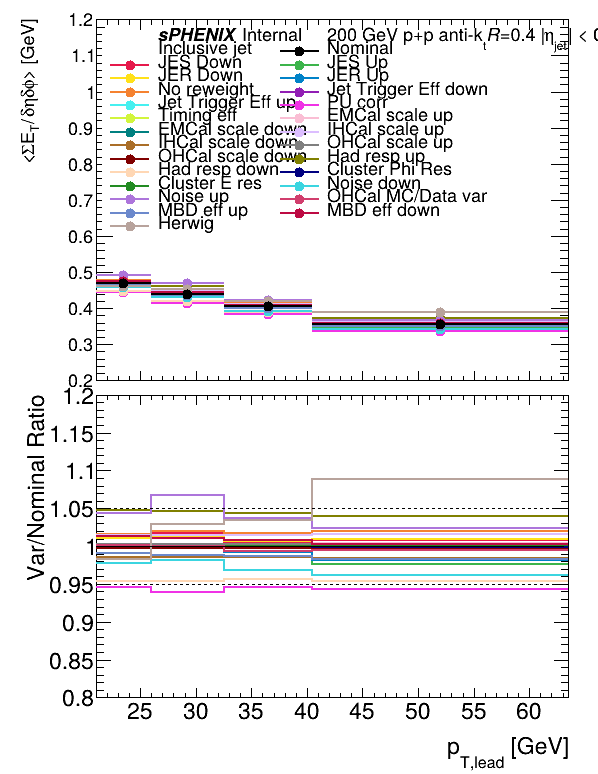
\includegraphics[width=0.48\linewidth]{ueinpp/Figures/h_profile_inclusive.png}
    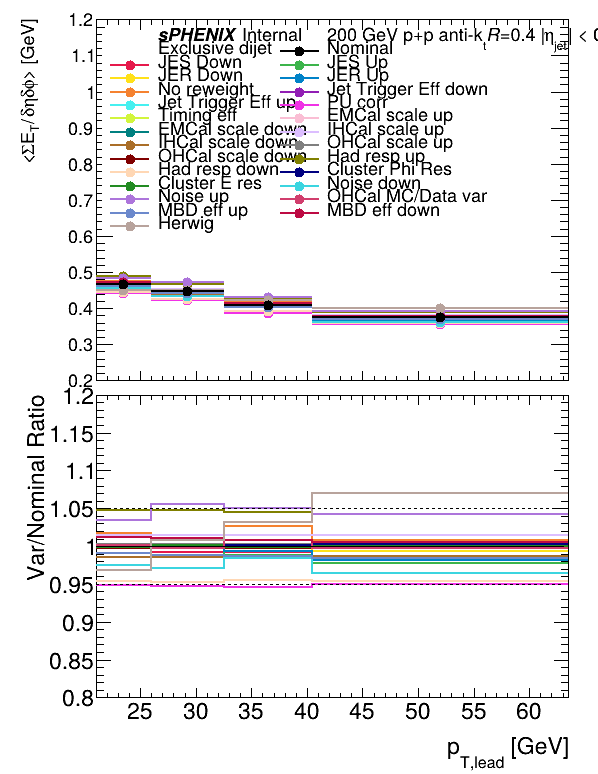
\includegraphics[width=0.48\linewidth]{ueinpp/Figures/h_profile_dijet.png}
    \caption{Total set of contributions to the systematic uncertainty on the UE measurement as a function of leading jet $p_T$ for inclusive jet (left) and dijet (right) events. Ratio of variations to nominal distribution shown in bottom panel.}
    \label{fig:total_systematic_uncertainty}
\end{figure}

The values of the systematic variations for the inclusive jet and dijet event results given in Figure \ref{fig:total_systematic_uncertainty} are averaged over the leading jet $p_{T}$ bins and are presented in Table \ref{table:systematics}.
\begin{table}[ht]
\centering
\begin{tabular}{|c|c|c|}
\hline
Systematic Uncertainty & Inclusive Jet Variation & Dijet Variation \\ \hline
JES Down & 2.5\% & 3.62\% \\ \hline 
JES Up & -2.02\% & 1.75\% \\ \hline 
JER Down & -1.47\% & 2.82\% \\ \hline 
JER Up & -2.6\% & -1.43\% \\ \hline 
No reweight & 2.7\% & 4.6\% \\ \hline 
Jet Trigger Eff down & 0.00231\% & 0.00236\% \\ \hline 
Jet Trigger Eff up & 0.0036\% & 0.00446\% \\ \hline 
PU corr & -3.97\% & -4.48\% \\ \hline 
Timing eff & 0\% & 0\% \\ \hline 
EMCal scale up & 0.34\% & 0.368\% \\ \hline 
EMCal scale down & -0.224\% & -0.288\% \\ \hline 
IHCal scale up & 1.55\% & 1.43\% \\ \hline 
IHCal scale down & -1.32\% & -1.26\% \\ \hline 
OHCal scale up & 0.367\% & 0.41\% \\ \hline 
OHCal scale down & -0.245\% & -0.225\% \\ \hline 
Had resp up & 5.82\% & 6.08\% \\ \hline 
Had resp down & -5.57\% & -5.29\% \\ \hline 
Cluster Phi Res & 0.102\% & 0.129\% \\ \hline 
Cluster E res & 1.01\% & 1.64\% \\ \hline 
Noise & 2.53\% & 3.62\% \\ \hline 
OHCal MC/Data var & -0.709\% & 0.958\% \\ \hline 
MBD eff up & -1.7\% & -1.75\% \\ \hline 
MBD eff down & 1.25\% & 1.16\% \\ \hline 
\end{tabular}
\caption{Detailed values of the jet $p_{T}$ bin-averaged systematic uncertainty for inclusive jet and dijet events.}
\end{table}
\label{table:systematics}
